
% Subsection '2a'
% Tier 0 and Tier 1's
%
%\subsection{Deployment at the Tier-0 and Tier-1 sites}
%Efforts were made to investigate whether the WLCG software packages could be enabled to run in a dual-stack environment or even become protocol agnostic. The first software packages that were examined were data transfer software packages like FTS and SRM. After the examination some software packages were replaced like AFS with EOS, or CASTOR with DPM. Today the storage environment is dual/stack ready and at CERN the Tier-0 is IPv6 and IPv4 dual-stack enabled. The Tier-1 sites: CA-Triumf, DE-KIT, ES-PIC, FR-CCIN2P3, IT-INFN-CNAF, NDGF, NL-T1 (SARA-Matrix and NIKHEF), RRC-JINR-T1, TW-ASGC, UK-T1-RAL, US-T1-BNL, US-T1-FNAL are dual-stack deployed as shown in the following figure. ~\ref{fig:t1ds}.
%\begin{figure}[b]
%\centering
%\includegraphics[width=13cm]{Tier-1-IPv6-dual-stack}
%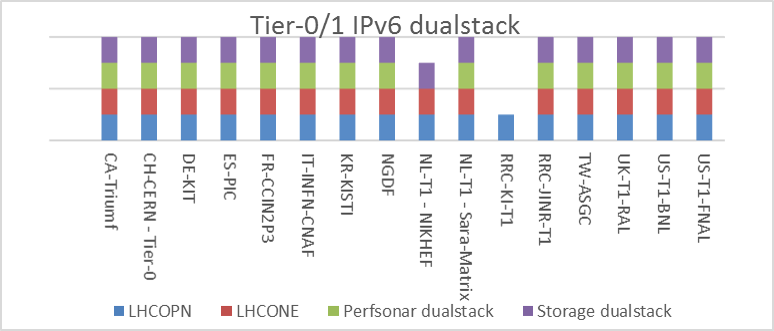
\includegraphics[width=13cm]{hepix-ipv6-tier01-dual-stack.png}
%\includegraphics[width=13cm]{t1ds}
%\caption{Tier-0/1 IPv4/6 dual-stack redyness incl dual-stack perfsonar server deployment}

\subsection{Deployment at Tier-0 and Tier-1's}
Efforts were made to investigate whether the WLCG software packages could be enabled to run in a dual-stack environment or even become protocol agnostic. The first software packages that were examined were data transfer software packages like FTS and SRM. After the examination some software packages were replaced like AFS with EOS, or CASTOR with DPM. Today the storage environment is dual/stack ready and at CERN the Tier-0 is IPv6 and IPv4 dual-stack enabled. The Tier-1 sites: CA-Triumf, DE-KIT, ES-PIC, FR-CCIN2P3, IT-INFN-CNAF, NDGF, NL-T1 (SARA-Matrix and NIKHEF), RRC-JINR-T1, TW-ASGC, UK-T1-RAL, US-T1-BNL, US-T1-FNAL are dual-stack deployed as shown in the following figure. ~\ref{fig:t1ds}.
\begin{figure}[h]
\centering
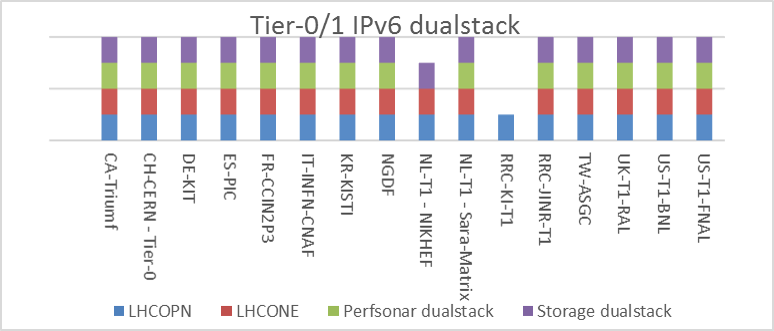
\includegraphics[width=6cm]{hepix-ipv6-tier01-dual-stack}
\caption{Tier-0/1 IPv4/6 dual-stack redyness incl. dual-stack perfsonar server deployment}
\label{fig:t1ds}
\end{figure}
But even while the IPv6 readiness deadline in April 2018 is long ago, there is one part of the Russian Tier-1 federation RRC-KI-T1 still deployed with IPv4 only. The dual-stack perfsonar server is deployed at almost all sites except NL-T1-NIKHEF and RRC-KI-T1. The FTS server at FNAL is still running in IPv4 prefered mode. There were a long standing malfunctioned transfer issue to IPv4 only US-Tier-2 sites which is solved now. This last server will get deployed in dual-stack as soon as possible.
